%!TEX root = ../nwoods_thesis.tex

\chapter{Object Reconstruction and Selection}\label{ch:reco}

The raw detector information stored on disk after an event passes trigger selections is not yet suitable for physics analysis.
Hits in the tracker and muon systems, and energy deposits in the calorimeters, require significant processing to build physics objects that are interpretable in terms of the physics of the hard scatter.
Patterns in the tracker and muon system hits are found and used to construct charged particle and muon tracks, and energy deposits in the calorimeters are grouped into clusters.
Final state particles that interact with CMS are reconstructed from the tracks and calorimeter clusters, final state particles are clustered into jets, charged particles are clustered by track origin to find proton-proton collision vertices, and visible particle momenta are summed to find the transverse momentum imbalance from undetectable particles (in the SM, neutrinos).
The resulting physics objects undergo selection to determine which represent real particles of interest for the analysis.
Selected particles are used to reconstruct the hard interaction from the collision---in the analyses presented here, leptons are paired to form {\Zgs} boson candidates which may be paired to form Higgs or {\PZ} boson candidates or nonresonant {\ZZ} candidates, and jets are used to construct hadronic observables and to distinguish electroweak and QCD {\ZZ} production.


\section{Track Reconstruction and Vertex Identification}\label{sec:trkVtxReco}

Tracks are reconstructed in the inner tracker by iterative application of a combinatorial Kalman filter algorithm~\cite{Fruhwirth:1987fm,Billoir:1990we,Adam:2005cg,Chatrchyan:2014fea}.
At each iteration, tracks found in the pixel detector are used as ``seeds'', track segments which serve as the initial trajectories on which strip tracker hits from the same particle are expected.
The pixel seed supplies the initial parameters for the combinatorial Kalman filter.
At each tracker layer, the algorithm predicts where the particle will hit the next layer based on the track's current parameters, taking into account the effects of particle interaction with tracker material.
The extrapolated trajectory is used to find compatible hits in the next layer with a $\chi^2$ test, and if possible the most compatible hit is added to the track and its parameters are updated accordingly.
If no hits are compatible, a ``ghost'' hit which does not contribute to the track parameters may be added to account for the possibility of a missing hit in the corresponding layer.
This procedure is repeated recursively at each tracker layer, from the innermost layer past the seed to the outermost layer of the silicon strip tracker.
If two tracks found in an iteration share too many hits, they are assumed to be from the same particle and the one with fewer hits is rejected, using the total $\chi^2$ of all hits as a tiebreaker.
The first iterations of the track finding algorithm searches for high-$\pt$ tracks from primary proton-proton interactions, which are easier to find because they are close to straight and originate from the beam line.
When a track is found, its constituent hits are removed from consideration in future iterations, reducing the computational complexity of finding the more difficult tracks from lower-$\pt$ particles and products of $\Pqb$~hadron decays which happen away from the beam line.

Because the Kalman filter obtains the final track parameters only at the outermost tracker layer, each track is refit and smoothed with further Kalman filters, improving track quality and reducing fake rate.
Spurious tracks are rejected from the final collection with requirements on the number of layers hit, the $\chi^2$ of the fit, and compatibility with a primary vertex.
The efficiency for reconstructing tracks of all prompt charged particles with $\pt > 900\MeV$ is around 94\% in the barrel and 85\% in the endcap; for isolated muons, it is virtually 100\% in the whole tracker acceptance~\cite{Chatrchyan:2014fea}.

Electrons lose substantially more energy to interactions with the tracker material than other charged particles, often breaking the assumption of Gaussian energy loss inherent to the Kalman filter.
To mitigate the impact of the resulting poor track fits, tracks with many missing hits or a poor $\chi^2$ are refit using a Gaussian sum filter (GSF)~\cite{Adam:2005bya}.
Any Kalman filter or GSF tracks with trajectories that intersect ECAL energy clusters (see below) are considered electron track candidates and refit with a second, more complicated GSF\@.
This GSF track collection is used as inputs to the PF electron reconstruction described below.

Proton-proton interaction vertices are found by clustering tracks by minimizing the figure of merit
\begin{equation}\label{eq:vtxChi2}
  \chi^2 = \sum_i \sum_j p_{ij} \frac{\left(z^t_j - z^V_i\right)^2}{\sigma_{j}^2},
\end{equation}
where $z^V_i$ is the $z$ position of vertex $i$, $z^t_j$ is the $z$ position of track $j$ at its closest point to the beamline, and $\sigma_j^2$ is its uncertainty.
The track-vertex association matrix $p_{ij}$ maps tracks to their associated vertices, i.e.\ $p_{ij} = 1$ if vertex $i$ and track $j$ are associated, $p_{ij} = 0$ if they are not.
Rather than minimize Eq.~(\ref{eq:vtxChi2}) directly with an unknown number of vertices, the CMS clustering algorithm~\cite{Speer:2006mh,Chatrchyan:2014fea} uses a technique known as deterministic annealing~\cite{Rose:726788}, which treats the system as a statistical ensemble of associations between the tracks and an unknown number of vertices.
The association matrix $p_{ij}$ is then the probability that vertex $i$ and track $j$ are associated.
If every possible set of assignments, for every possible number and arrangement of vertices, is considered equally probable, this is analogous to a thermodynamic system at high temperature, with $\chi^2$ playing the role of energy.
The system is simulated at high ``temperature'' and the analog of free energy is minimized to determine $p_{ij}$.
The temperature is then lowered in steps, with track-vertex associations deterministic in the limit of zero temperature.

Among the interaction vertices in an event, the one whose associated charged particles have the highest sum of $\pt^2$ is labeled the primary vertex (PV).
A PV must be less than 24\unit{cm} from the nominal beam spot in the $z$ direction and less than 2\unit{cm} from it in the $x$-$y$ plane.
Many commonly-used analysis observables are strongly dependent on the number of secondary proton-proton interaction vertices in the event, colloquially called the pileup.
The pileup distributions used in Monte Carlo samples are not the same as the distribution in data, biasing sensitive quantities.
Monte Carlo events are therefore reweighted based on the number of simulated pileup vertices such that the overall $N_\textit{vtx}$ (number of proton-proton interaction vertices) distributions match.



\section{Particle Flow Reconstruction}

The simplest conceivable algorithm would reconstruct each type of particle mostly with information from single subsystems: muons with the outer muon system, electrons and photons with ECAL (using HCAL to differentiate them from hadrons), jets with the calorimeters aided by inner tracker information to handle $\Pqb$ jet vertexing, etc.
This approach is sufficient for many analyses and sophisticated versions of the general principle have performed admirably at a number of experiments, but it is suboptimal.
It fails to exploit the full detector information for many objects---for example, not using the inner tracker's precise measurements of low-energy charged hadrons in jets made by clustering calorimeter deposits---and misses significant correlations between detector systems.
The CMS collaboration takes a different approach, using a particle flow (PF) algorithm combining subdetector signals for optimal particle reconstruction and identification~\cite{CMS:2009nxa,CMS:2010byl,Sirunyan:2017ulk}.

Several features of CMS facilitate PF reconstruction, as described in Section~\ref{sec:cms}.
The most important is that the calorimeters are inside the magnet and close to the tracker, so charged particles are much less likely to interact with material between them.
The inner tracker's precise position measurement and ECAL's fine segmentation thus allow tracks to be associated to calorimeter clusters even for individual charged hadrons of modest energy.

\subsection{PF Candidates}

The inputs to the PF algorithm are inner tracker tracks, muon system tracks, and clusters of energy deposits in the calorimeters, all of which are calibrated beforehand.
Calorimeter clusters are built independently for each subsystem, with ECAL and HCAL barrel and endcaps considered separately.
Topological clusters are built by combining adjacent cells with energy deposits over a threshold, using cells that are local energy maxima as seeds.
Within the topological clusters, the final calorimeter clusters are built by fitting the energy deposits with the sum of several two-dimensional Gaussians, one Gaussian for each seed in the topological cluster.

The first step of the PF algorithm is to link tracks and clusters across subdetectors.
Tracks are linked to calorimeter clusters by extrapolating from the track to the calorimeter cells the particle would be expected to hit.
To account for bremsstrahlung photons from electron interactions with tracker material, GSF tracks are linked with ECAL clusters compatible ($\Delta\eta < 0.05$) with a tangent to the track where it hit the tracker.
Overlapping ECAL and HCAL clusters are linked outside the inner tracker acceptance.
Inner tracks are linked to muon system tracks if their hits can be propagated onto a common surface and merged into a single track within the resolution of the muon system (see Section~3.3 of Ref.~\cite{Sirunyan:2017ulk}).
The groups of linked objects, called ``PF blocks'', usually originate from one or a few particles and are the basic unit of PF reconstruction.

\subsubsection{Muons}

Muon candidates in CMS~\cite{Chatrchyan:2012xi} come in three flavors: ``standalone'', ``tracker'', and ``global'' muons.
Standalone muons use only the track from the muon spectrometer (the ``standalone track''), built with a fit to track segments made of clusters of hits in the DTs, CSCs, and RPCs.
Tracker muons use only the inner track, identified as a muon because the track is compatible with one or more track segments in the muon system within {3\unit{cm}} transverse to the track direction, or four standard deviations of the track's angular position uncertainty.
Global muons use a combined ``global track'' made by fitting the hits in an inner track and a compatible standalone track to a common muon trajectory through the whole detector.
By construction, global muons have corresponding standalone and tracker muons.
Tracker muons are merged into their corresponding global muons, which use the inner track momentum for muons with $\pt < 200\GeV$ and the momentum of the track with the best normalized $\chi^2$ otherwise.
When a muon candidate is reconstructed, its constituent tracks are removed from the PF block and are therefore not used in further reconstruction.

\subsubsection{Electrons and Prompt Photons}

Electron reconstruction uses GSF tracks linked with ECAL clusters~\cite{Baffioni:2006cd,Adam:2005bya}.
The cluster associated with a track and the bremsstrahlung candidate clusters on tangents to the track are collectively called the ``supercluster''.
Prompt photons are reconstructed from superclusters without associated tracks except displaced track pairs consistent with photon-initiated electron-positron pair production in the tracker material~\cite{Khachatryan:2015iwa}.
In both cases, the HCAL energy near the supercluster cannot be more than 10\% of the supercluster energy.
Non-isolated photons, i.e.\ those with substantial nearby tracks or calorimeter deposits or a high ratio of HCAL energy to ECAL energy, are assumed to be from $\pi^0$ decays and are described with neutral hadrons in the next section.
Tracks and clusters used to reconstruct electrons and photons are removed from the PF block and are not used in hadron reconstruction.


\subsubsection{Charged and Neutral Hadrons}

With muon, electron, and prompt photon constituents removed, remaining detector signals are taken to be from charged and neutral hadrons (including non-prompt photons)~\cite{CMS:2009nxa,Sirunyan:2017ulk}.
Clusters in ECAL without associated tracks are taken to be photons from $\pi^0$ decays, because neutral hadrons deposit very little energy in ECAL\@.
Trackless clusters in HCAL are taken to be neutral hadrons.
Both are removed from the PF blocks, so all that remain are linked clusters and tracks.
Paired tracks and clusters with compatible energies are taken to be charged hadrons.
If the track {\pt} is much less than the calorimeter-measured {\pt}, the pair is labeled as overlapping charged and neutral hadrons.


\subsection{Jets}

Effective clustering of hadrons, non-prompt photons, and non-prompt leptons into jets is critically important for many physics analyses, including the $\ZZ + \text{jets}$ differential cross section measurements and the {\ZZ} VBS search (see Sections~\ref{sec:vbsSearch} and~\ref{sec:vbsSelection}).
Clustering must be efficient, to ensure the tagging jets in VBS events are found, but the clustering algorithm should not tag spurious jets, as the number of jets in an event is sensitive to higher-order QCD corrections and therefore an interesting quantity to compare to theoretical predictions.
Similarly, the algorithm should not erroneously cluster particles from the same initial parton into multiple jets or merge jets from multiple original partons, because the kinematics of the original quarks and gluons are also of theoretical interest and the detector-level jet kinematics should accurately reflect them.
A clustering algorithm is said to be ``infrared safe'' if the presence of low-energy hadrons from soft gluon radiation does not change the number of jets or have a qualitatively significant effect on jet shapes and kinematics.
This fits with the intuition that a single {1\GeV} pion should have essentially no effect in an event with multiple jets with energies on the order of hundreds of {\GeVns}~\cite{Salam:2007xv}.
An algorithm is said to be ``collinear safe'' if the jets are not changed substantially by splitting one hadron into two nearly collinear hadrons with the same total four-momentum.
This also fits with physical intuition in that jets deposit energy over an area significantly larger than the spatial resolution of the detector, so increasing the detector granularity enough to resolve two very close particles (without changing their total four-momentum) should have little or no effect on the jet.

Infrared and collinear (IRC) safety are critically important for comparing data to theoretical predictions~\cite{Salam:2009jx}.
Collinear splittings and soft gluon radiation during jet fragmentation should not affect the dynamics of the {\TeVns}-scale hard scattering processes we wish to probe, but they are nonperturbative and difficult to model (see Section~\ref{sec:partonShower}), and experimental analysis can only probe the underlying hard interaction if it is insensitive to this kind of mismodeling.
Experimental detectors' finite resolution and inability to measure arbitrarily soft particles enforces some level of IRC safety on any algorithm, but the results of an analysis methods that uses an IRC unsafe clustering will depend on the complex, detector-dependent details of this partial IRC regularization.
In any case, the most meaningful comparisons between data and theory should use the same definition of a jet in the experimental analysis and the perturbative calculation, and perturbative calculations require IRC safe observables to preserve unitarity.

These considerations, and the desire for conical jets with a well-defined area in the $\eta$-$\phi$ plane, lead most CMS analyses (including this one) to use jets clustered with the anti-{\kt} algorithm~\cite{Cacciari:2008gp,Cacciari:2011ma}.
The anti-{\kt} algorithm defines the distance between two particles $i$ and $j$ as
\begin{equation}
  d_{ij} = \min\left(p_{\text{T}i}^{-2}, p_{\text{T}j}^{-2}\right) \frac{\Delta_{ij}}{R},
\end{equation}
where $\Delta_{ij}$ is the distance in the rapidity-polar angle plane,
\begin{equation}
  \Delta_{ij}^2 \equiv \left(y_i - y_j\right)^2 + \left(\phi_i - \phi_j\right)^2,
\end{equation}
and $R$ is a parameter setting the size of the resulting jets.
The algorithm proceeds iteratively.
At each iteration, if the smallest $d_{ij}$ between any pair of particles in the event is smaller than the smallest $\pt^{-2}$ of any single particle, the particles in the pair are merged into a single particle with their total four-momentum.
If the minimum single-particle $\pt^{-2}$ is smaller than the minimum $d_{ij}$, the single particle is labeled a jet and removed from further consideration.
Iteration proceeds until all particles are part of a jet.
In this analysis, the size parameter used is $R = 0.4$.

Charged hadrons whose tracks originate in pileup interactions are not included in jet clustering~\cite{CMS:2014ata}.
The contribution of neutral hadrons from pileup is estimated with a jet area technique~\cite{Khachatryan:2016kdb,Cacciari:2008gn,Cacciari:2007fd} in which the energy density of neutral hadrons from pileup is calculated event-by-event and multiplied by the area of the jet to estimate the neutral pileup contribution, which is subtracted from the jet energy.
Jets in Monte Carlo samples have their energy shifted and stochastically smeared such that the overall energy scale and resolution match that of jets in data~\cite{Chatrchyan:2011ds,Khachatryan:2016kdb}.


\subsection{Missing Transverse Energy}

Neutrinos---or, hypothetically, WIMP dark matter or other new particles that do not decay or interact directly with the detector---escape and cannot be directly measured.
Because the beams have no momentum in the $x$-$y$ plane, the transverse momentum of the visible particles must balance the transverse momentum of the invisible ones.
The missing transverse momentum is thus
\begin{equation}\label{eq:MET}
  \ptvecmiss = -\! \! \sum_\text{visible} \ptvec,
\end{equation}
where the sum runs over the transverse momenta of all PF candidates in the event.
The missing transverse energy, {\MET}, is its magnitude.
The {\MET} is calibrated by propagating the jet energy scale corrections to the {\MET} calculation~\cite{Chatrchyan:2011tn,Khachatryan:2014gga,CMS-PAS-JME-16-004}.
All PF candidates are included in the sum in Eq.~(\ref{eq:MET}), including those originating from pileup interactions, because these soft collisions are very unlikely to produce neutrinos, so including them biases the measurement less than trying to determine which neutral particles should be considered pileup and which should not.



\section{Object Identification and Selection}

The reconstruction algorithms described above are general purpose in the sense that they can be used in nearly any analysis, but do not address the specific needs of any, so further selections are essentially always required to optimize object efficiency and purity for studying a specific physics process.
The leptons used in this analysis are required to pass identification requirements on top of those imposed during PF reconstruction, and are required to be isolated from other particles in the event, to reject fake objects from jet fragmentation.
Four-lepton processes have low reducible backgrounds, so the selections presented here are generally loose, optimized for high efficiency compared to most CMS analyses.


\subsection{Electrons}

Electrons are required to have $\pt > 7\GeV$ and to be in the tracker acceptance, $\abseta < 2.5$.
They must be compatible with the PV, with minimum track-PV distance $d_z < 1\unit{cm}$ in the $z$ direction and $d_{xy} < 5\unit{mm}$ in the plane transverse to the beam.
Each electron's 3-dimensional impact parameter (IP) $d_\text{3D}$ must satisfy a requirement on its significance,
\begin{equation}
  \text{SIP}_\text{3D} \equiv \frac{d_\text{3D}}{\sigma_{d_\text{3D}}},
\end{equation}
where $\sigma_{d_\text{3D}}$ is the uncertainty on the IP\@.
The $\text{SIP}_\text{3D}$ requirement is $\text{SIP}_\text{3D} < 10$ for the {\ZZ} and {\Zfourl} cross section measurements and the aTGC search, and $\text{SIP}_\text{3D} < 4$ for the Higgs boson measurement and the VBS and aQGC searches.
Distributions of $\text{SIP}_\text{3D}$ are shown for electrons and muons in Fig.~\ref{fig:lepton_sip}.
To remove fake electrons arising from muon tracks being associated to photons or other incidental ECAL energy clusters, electrons within $\Delta R < 0.05$ of a muon are vetoed.

\begin{figure}[htbp]
  \begin{center}
    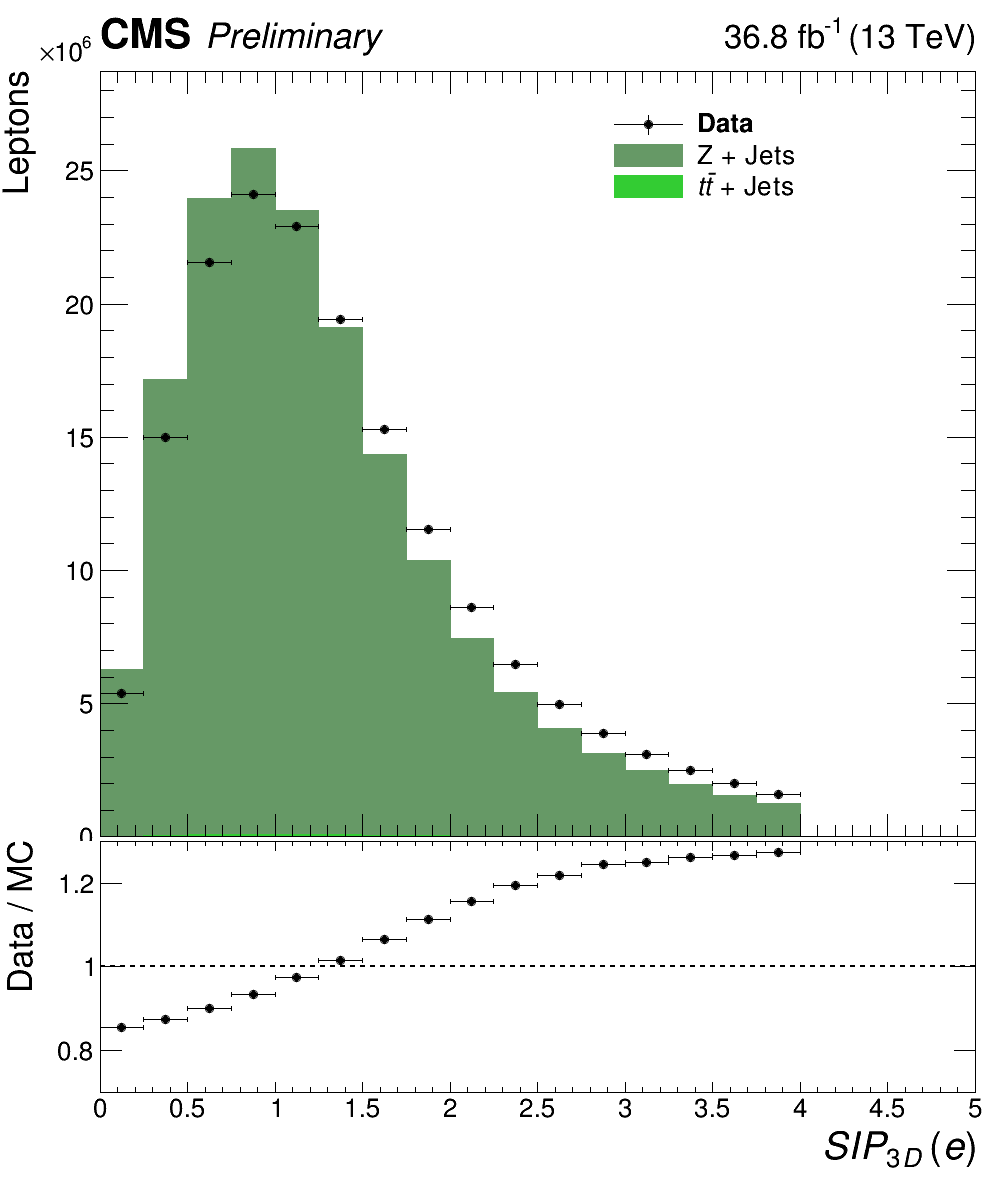
\includegraphics[width=0.45\textwidth]{objects/eSIP3D.png}
    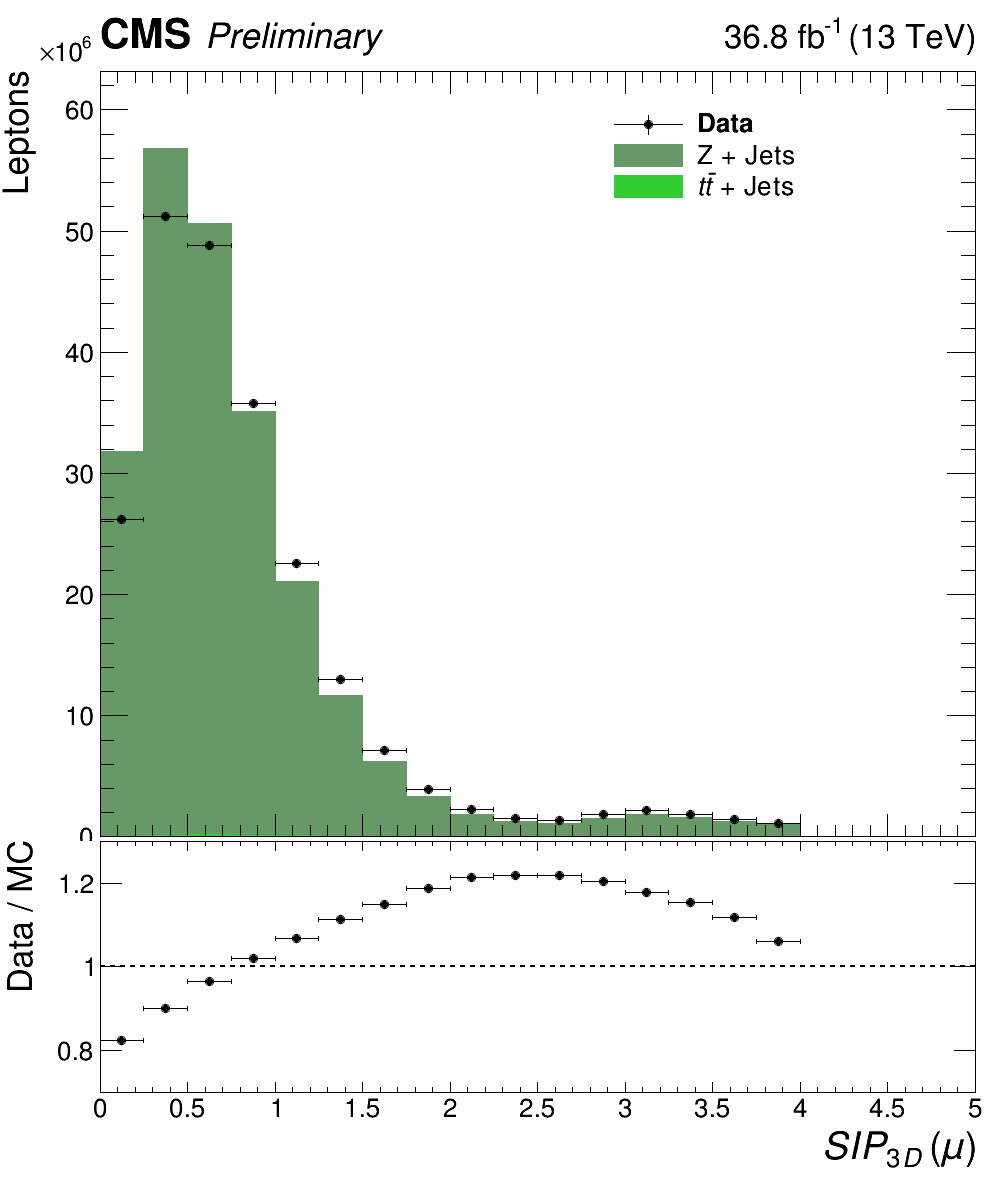
\includegraphics[width=0.45\textwidth]{objects/mSIP3D.png}
    \caption[Lepton vertex compatibility]{
      Vertex compatibility in the form of the $\text{SIP}_\text{3D}$ distribution for electrons (left) and muons (right) in a single-{\PZ} sample.
      The distribution extends only to 4 because these events were used for Higgs boson measurements.
      }\label{fig:lepton_sip}
  \end{center}
\end{figure}

To further reduce photon and jet fragment backgrounds while maintaining high prompt electron efficiency, a further selection is applied using a multivariate discriminator made with a boosted decision tree (BDT)~\cite{CMS:2010bta,Khachatryan:2015hwa}.
The BDT uses 21 input variables, which fall into three broad categories:
\begin{itemize}
  \item Track-related observables like the number of hits and normalized $\chi^2$ of the Kalman and GSF tracks and the energy lost to bremsstrahlung according to the GSF fit. These are intended to discriminate between electrons and charged hadrons.
  \item Calorimetric information including a number of supercluster shape observables and the amount of HCAL energy near the supercluster, to discriminate electrons from electromagnetically rich jets.
  \item Track-cluster observables comparing the positions and momenta of the particles seen in the tracker and by ECAL\@.
\end{itemize}
The BDT training and working point selection are done separately for electron candidates with {\pt} above and below {10\GeV} and in three bins of {\abseta} (0--0.8, 0.8--1.479, and 1.479--2.5).
The working points are chosen to correspond to 98\% efficiency for single signal electrons in each bin.

To ensure that electron candidates are not part of a jet, they are required to be isolated from other particles in the event.
The relative isolation is defined as
\begin{equation}\label{eq:iso}
  R_\text{Iso} = \left( \sum_\text{charged} \! \!\pt + \max\left[0, \sum_\text{neutral} \! \!\pt + \sum_{\text{photons}} \! \!\pt - \pt^\text{PU} \left(\ell\right) \right]\right) \bigg/ \pt^{\ell}
\end{equation}
where the sums run over the {\pt} of PF hadrons and photons in a cone of $\Delta R < 0.3$ around the electron trajectory.
To mitigate the contribution of pileup to the isolation calculations, charged hadrons are included only if they originate from the event's PV\@.
The estimated neutral contribution to isolation from pileup, $\pt^\text{PU}\left(\ell\right)$, is defined for electrons as
\begin{equation}
  \pt^\text{PU}\left(\Pe\right) \equiv \rho \times A_\text{eff},
\end{equation}
where the average transverse-momentum flow density $\rho$ is calculated in each event using the jet area method described above.
The effective area $A_\text{eff}$ is the geometric area of the isolation cone times an $\eta$-dependent correction factor that accounts for the residual dependence of the isolation on pileup.
Electrons are considered isolated if their relative isolations satisfy $R_\text{iso} <0.35$.
Relative isolation distributions are shown for electrons and muons in Fig.~\ref{fig:lepton_iso}.

\begin{figure}[htbp]
  \begin{center}
    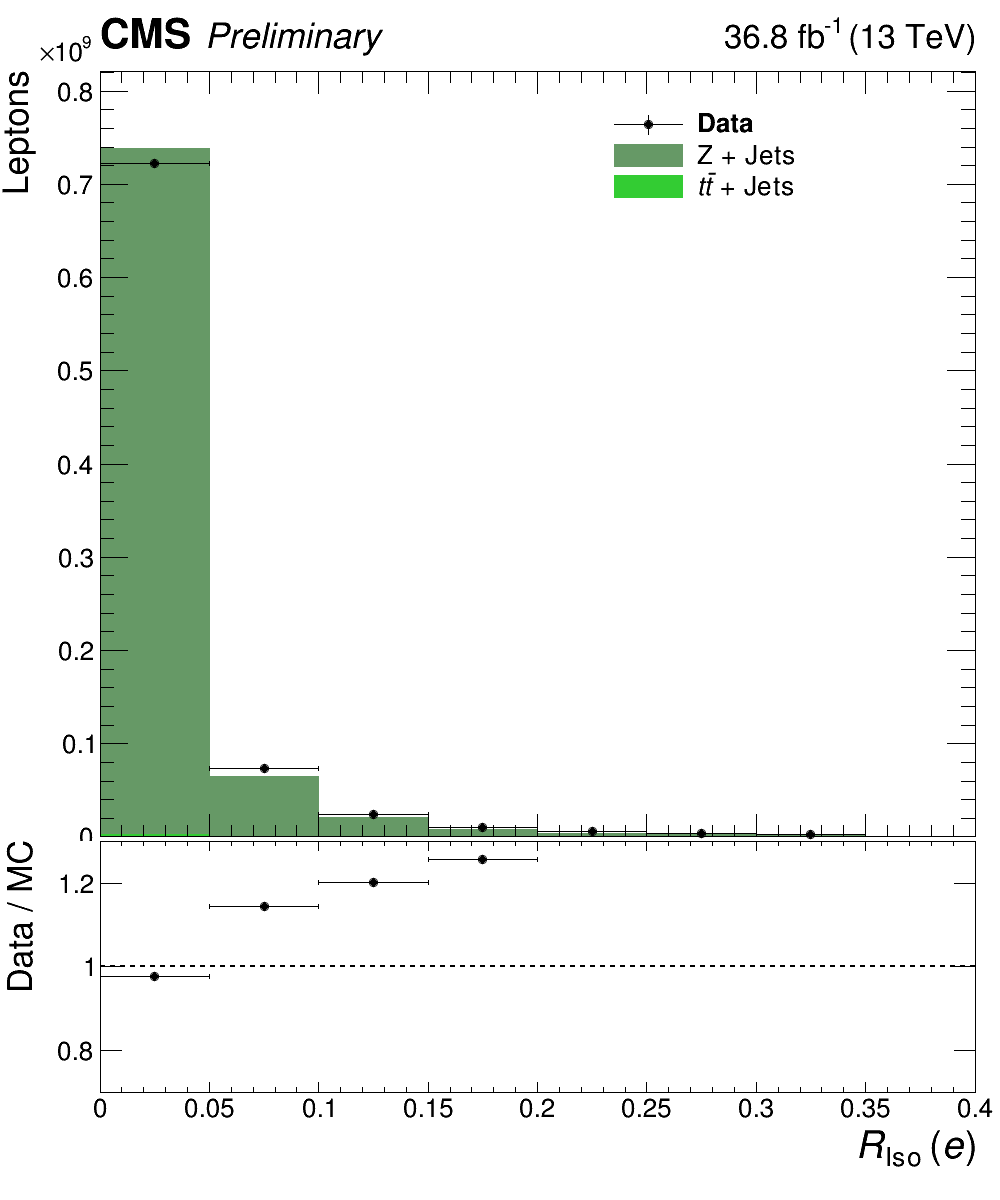
\includegraphics[width=0.45\textwidth]{objects/eIso.png}
    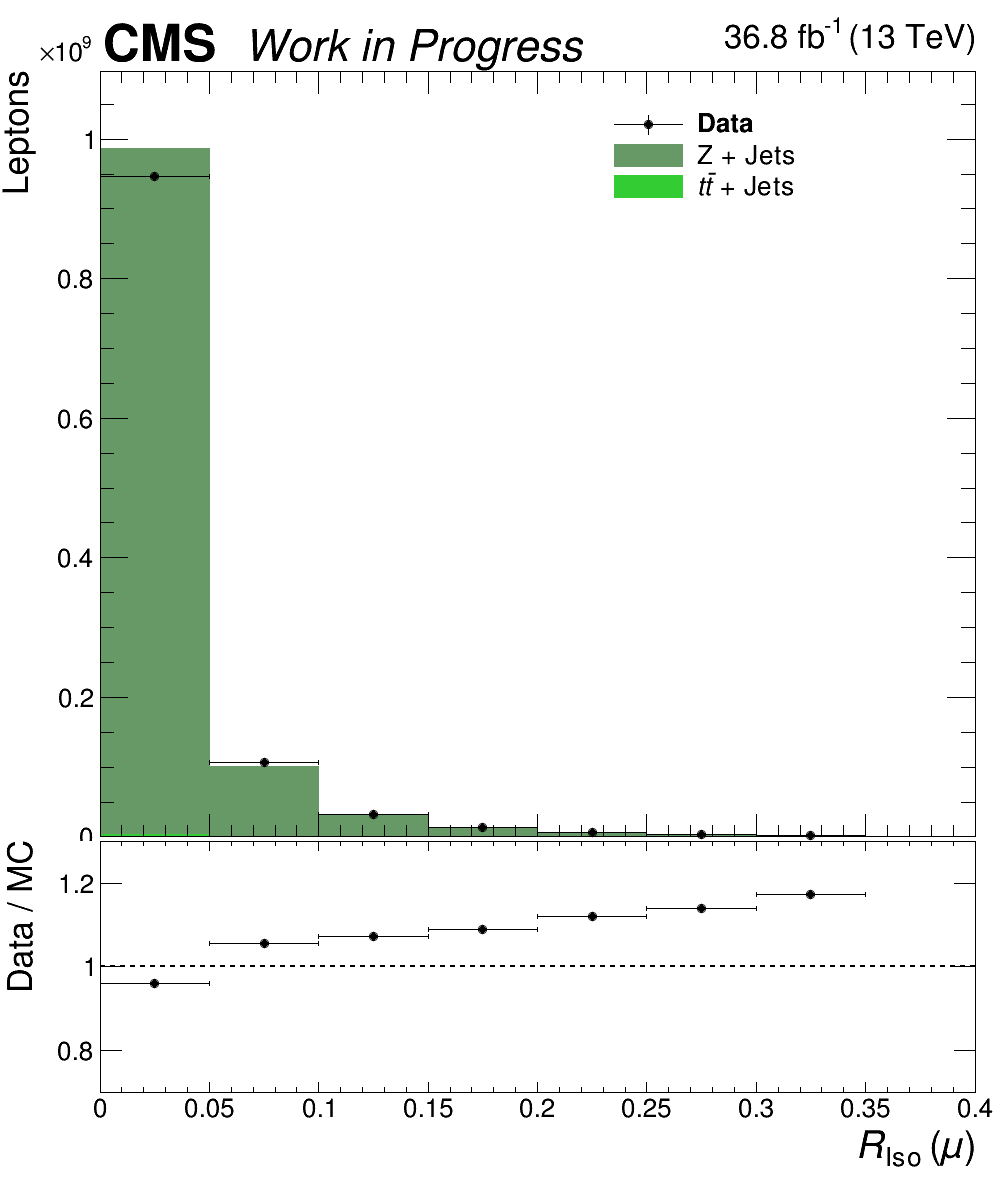
\includegraphics[width=0.45\textwidth]{objects/mIso.png}
    \caption[Lepton isolation distributions]{
      Relative isolation for electrons (left) and muons (right) in single-{\PZ} events.
      }\label{fig:lepton_iso}
  \end{center}
\end{figure}

Efficiencies for GSF track reconstruction, electron reconstruction and identification, and electron isolation criteria, are found with a ``tag-and-probe'' method~\cite{CMS:2011aa}.
In this technique, events are selected which contain at least one high-{\pt} ``tag'' electron passing strict ID and isolation requirements, and a ``probe'' track with the opposite sign that combines with the electron to have an invariant mass close to the {\PZ} boson mass.
The resulting sample is enriched with $\PZ \to \Pe^+\Pe^-$ events, so the track is likely to correspond to a real prompt electron.
Unlike all background processes, $\PZ \to \Pe^+\Pe^-$ production forms a distinct resonance peak in the $m_{\ell\ell}$ distribution, so shape fits can be used to find the overall purity of the sample, and thus the number of prompt electrons among the probes.
The selection efficiency is then the number of passing probes divided by the total number of prompt probes.
This procedure is performed in bins of {\pt} and $\eta$ for data and Monte Carlo events, and residual differences in efficiency in Monte Carlo samples are corrected to match data by weighting events by the ratio of data and Monte Carlo efficiency for each electron candidate.
Overall electron efficiency varies between roughly 85\% in the inner endcap ($\abseta > 2.0$) to around 95\% in the central barrel ($\abseta < 0.8$).


\subsection{Muons}

Muon selection is similar to electron selection, but simpler because muon backgrounds are much smaller.
Candidate muons are required to be tracker or global muons with $\pt > 5\GeV$  within the muon system acceptance ($\abseta < 2.4$).
They are subject to the same PV compatibility criteria as electrons, $d_z < 1\unit{cm}$, $d_{xy} < 5\unit{mm}$, and $\text{SIP}_\text{3D} < 10$ or 4 depending on the analysis.
Muon candidates are further subject to the so-called ``PF ID'' criteria, which require them to be isolated from calorimeter deposits or to have high-quality tracks with good fits~\cite{Sirunyan:2017ulk}.

Isolation is defined as in Eq.~(\ref{eq:iso}), the same as for electrons except for the definition of the neutral pileup contribution, which for muons is based on using the known charged pileup density to estimate the neutral pileup based on the average charge composition of pileup jets,
\begin{equation}
  \pt^\text{PU}\left(\Pm\right) \equiv 0.5 \sum_\text{charged} \pt^\text{PU},
\end{equation}
where the sum runs over the charged particles from all pileup vertices.
As for electrons, the radius of the isolation cone is 0.3 in the $\eta$-$\phi$ plane and the selection criterion is $R_\text{iso} < 0.35$.
Muon efficiencies are measured and corrected with the same tag-and-probe technique as used for electrons, and found to be around 97\%.


\subsection{Final State Photon Radiation}

Final-state radiation (FSR) photons emitted by muons are not included in the PF momentum reconstruction, and some photons emitted by electrons may be missed, degrading {\PZ} boson reconstruction.
Photons are considered FSR candidates if they have $\pt > 2\GeV$, $\abseta < 2.4$, relative isolation $R_\text{iso} < 1.8$ as defined in Eq.~(\ref{eq:iso}) (with no neutral pileup correction), and $\Delta R \left(\ell, \gamma \right) < 0.5$ with respect to the nearest lepton.
To avoid double counting, photons in electron superclusters are not considered.
Because FSR has a higher energy spectrum than photons from pileup and is expected to be quasi-collinear with the emitting leptons, a photon is accepted as FSR and included in the {\ZZ} final state if $\Delta R \left( \ell, \gamma \right) / {\et}_\gamma^2 < 0.012$.
The performance of this algorithm is tuned and evaluated with comparisons to generator-level information in MC samples, and is found to have efficiency around 60\% for a purity around 80\%.
FSR photons are omitted from the isolation determination for emitting leptons.
In the rest of this thesis, the momentum of any FSR photons found is included in {\Zgs} and {\ZZ} four-momenta unless otherwise stated.


\subsection{Jets}

Jets are considered for analysis if they have $\pt > 30\GeV$ and $\abseta < 4.7$.
Loose criteria are applied to reject spurious jets by requiring they contain multiple particles, and the particles be a mix of charged and neutral consistent with hadronic jets.
Jets are removed from consideration in the event if a lepton or FSR photon is in its cone ($\Delta R < 0.4$ with respect to the jet's total momentum vector).


\subsection{Misidentified Objects}\label{sec:looseID}

The reducible background estimation method described in Section~\ref{sec:bkg} requires the use of ``loose'' lepton candidates which are similar to candidates passing the full selection but much more likely to be jet fragments or other non-prompt objects.
Loose lepton candidates pass the {\pt} and $\eta$ cuts and vertex compatibility criteria, but the other identification criteria are reduced.
The electron BDT discriminator is not applied to loose electrons.
Loose muons must still be tracker or global muons, but the PF ID is not applied.
Isolation requirements are not applied to loose candidates.
Depending on their use, loose candidates may have no further requirements applied, or may be required to fail the tight ID and/or isolation requirements, as detailed in Section~\ref{sec:bkg}, where the fake rates for electrons and muons are shown in Fig.~\ref{fig:fakerates}.
Aside from the ID and isolation criteria, loose leptons are treated the same as their tight cousins, with FSR recovery performed with the same algorithm.
Jets near loose leptons are only removed if the loose lepton is taken to be one of the four in the {\ZZ} candidate in the final event interpretation.



\section{ZZ Candidate and Event Selection}\label{sec:zzSelection}

Online event selections used single, double, and triple lepton triggers.
The double lepton triggers were the primary paths, with single and triple lepton triggers correcting for residual inefficiencies to bring the overall trigger efficiency above 99\%.
Exact HLT parameters changed over the course of datataking as instantaneous luminosities changed and trigger rates rose, so many thresholds are shown here as ranges.
\begin{itemize}
  \item Single muon {\pt} thresholds were between 20 and {24\GeV} for isolated muons.
  Nonisolated single muons were required to have $\pt > 50\GeV$ or $\pt > 45\GeV$ and $\abseta < 2.1$.
  Single electron {\pt} thresholds were 25 or {27\GeV} depending on ID criteria applied.
  \item Leading lepton {\pt} thresholds in double lepton paths were 17 or {23\GeV}.
  Trailing lepton thresholds were {12\GeV} and {8\GeV} for electrons and muons, respectively.
  Isolation requirements and requirements on the $z$-axis distance between lepton track origins were added part way through datataking.
  \item The {\pt} requirements in triple lepton paths varied between 5 and {16\GeV}, with no isolation or vertex requirements.
\end{itemize}
An event is considered for the analysis is any of these triggers fires.

Several distinct analyses fall under the four-lepton umbrella, each with different requirements and therefore different selection criteria.
The sets of selections will be listed here with brief descriptions of their uses, and detailed in full below.
\begin{itemize}
  \item The \emph{full spectrum selection} picks a phase space that encompasses all four-lepton events, and all other selection sets yield strict subsets of the full spectrum phase space.
  \item The \emph{singly resonant} ({\Zfourl}) \emph{selection} picks events with four-lepton mass around the {\PZ} boson resonance.
  \item The \emph{Higgs selection} is that used for the Higgs boson discovery and properties measurements.
  It is similar to the full spectrum selection but with slightly tighter requirements on the second {\Zgs} candidate, because {\Zfourl} events are of less interest and some backgrounds may be reduced by excluding events with an on-shell {\PZ} boson and a low mass lepton pair that could be a decay of an {$\Upsilon$} or similar meson.
  \item The \emph{on-shell} or \emph{doubly resonant selection} requires both {\PZ} candidates to be compatible with a resonant {\PZ} boson.
  It is used for the {\ZZ} and $\ZZ + \text{jets}$ cross section measurements and the aTGC search.
  \item The \emph{dijet} ({\ZZjj}) \emph{selection} uses the on-shell selection for the four-lepton system, and additionally requires at least two jets.
  It is used for the VBS and aQGC searches.
\end{itemize}


\subsection{\texorpdfstring{$\text{Z}/\gamma^\ast$}{Z/gamma*} Candidate Selection}\label{sec:zSelection}

A {\Zgs} candidate is built from a pair of opposite-sign, same-flavor leptons with invariant mass between 4 and {120\GeV}.
The {\Zgs} candidate with mass closest to the nominal {\PZ} boson mass is labeled $\PZ_1$, the other is labeled $\PZ_2$.
Mass requirements on the {\Zgs} candidates are among the primary differences between the various analysis selections.
The full spectrum, {\Zfourl}, and Higgs selections require $m_{\PZ_1} > 40\GeV$.
The Higgs selection additionally requires $m_{\PZ_2} > 12\GeV$.
The on-shell and dijet selections require both $\PZ_1$ and $\PZ_2$ to have $m_{\PZ_i} > 60\GeV$.
The mass range thus allowed, $60 < m_{\PZ_{1,2}} < 120\GeV$, serves as the definition of an on-shell {\PZ} boson for purposes of this analysis.

\begin{table}[htbp]
  \begin{center}
    \caption[Four-lepton event yields in data at several points in the analysis flow.]{
      The number of events in data reconstructed as having two pairs of opposite-sign, same-flavor leptons, at several points in the analysis flow.
      Best candidate selection is done only with the full spectrum selection, and an event may have candidates in multiple channels, so channel yields do not sum to the total yield in early steps.
    }\label{tab:cut_flow}
    \begin{tabular}{ccccc}
      \toprule
      Selection         &  $4\Pe$  &  $2\Pe2\Pm$  &  $4\Pm$  &  Total    \\
      \midrule
      \midrule
      Trigger           &  580633  &  645640      &  399212  &  1598705  \\
      Lepton ID         &  2195    &  6760        &  11614   &  20563    \\
      Lepton Isolation  &  597     &  1189        &  1548    &  3334     \\
      \midrule
      Full Spectrum     &  440     &  1111        &  838     &  2389     \\
      \midrule
      \midrule
      {\Zfourl}         &  78      &  206         &  225     &  509      \\
      \midrule
      \midrule
      {\Hfourl}         &  19      &  41          &  34      &  94       \\
      \midrule
      \midrule
      {\ZZfourl}        &  220     &  543         &  335     &  1098     \\
      \bottomrule
    \end{tabular}
  \end{center}
\end{table}


\subsection{ZZ Candidate Selection}

Four-lepton candidates are built from pairs of {\Zgs} candidates.
Among the four leptons in the candidate, all opposite-sign pairs must have invariant mass $m_{\ell^+\ell^{\prime -}} > 4\GeV$ regardless of flavor, to remove events in which decay products of a light, leptonically decaying particle like a {\PJpsi} are erroneously paired with the two leptons from a real {\PZ} boson to form two false {\Zgs} candidates by chance when paired incorrectly.
The requirement on all pairs does not include FSR photons, because the mesons that would cause such a problem are generally found in jets which include photons from $\pi^0$ decays, whcih are likely to be misidentified as FSR\@.
All lepton pairs must have $\Delta R > 0.02$ to avoid ``ghost'' leptons with shared tracks.
The leading and lepton among the four must have $\pt > 20\GeV$, and the subleading lepton must have $\pt > 10\GeV$ if it is an electron or $\pt > 12\GeV$ if it is an electron.
The {\Zfourl} selection requires the candidate to have $80 < m_{4\ell} < 100\GeV$, consistent with resonant single-{\PZ} production.

All allowed pairings of leptons into {\Zgs} candidates are examined separately, so an event with two electrons and two positrons, for example, will yield two possible {\ZZ} candidates, with the only difference being how the electrons are paired into $\PZ_1$ and $\PZ_2$.
In the case that multiple interpretations of the same event pass the full selection, the one with $\PZ_1$ closest to the nominal {\PZ} mass is chosen.
In the rare case of further ambiguity, which may arise in events with five or more leptons, $\PZ_2$ is chosen to maximize the scalar {\pt} sum of the four leptons.
This best candidate selection is done after the full selection is applied, and the other analysis selections are applied to the disambiguated events in the full spectrum phase space.
Like the mass cut on all opposite-sign lepton pairs, this prevents events with one on-shell {\PZ} and one lower-mass $\Pa^\ast$ from passing the on-shell {\PZ} mass cuts with an erroneous lepton pairing.

The number of events found in data after several analysis steps is shown in Table~x.
Specifically, the numbers in Table~x include events with four objects reconstructed as two opposite-sign, same-flavor lepton pairs.
Early in the analysis flow, most of these objects are fakes later removed by lepton ID and isolation requirements.
The total signal efficiency of all selections is estimated by finding the fraction of events in the {\POWHEG} and {\MCFM} {\ZZ} samples which pass both the fiducial cuts at generator level and the full analysis selection after detector simulation and reconstruction.
For the doubly on-shell selection ($60 < m_{\ell\ell} < 120\GeV$), the efficiency is 54\% for $4\Pe$ events, 65\% for $2\Pe2\Pm$ events, and 78\% for $4\Pm$ events.
For {\Zfourl} events, the efficiencies for the $4\Pe$, $2\Pe2\Pm$, and $4\Pm$ channels are, respectively, 24\%, 36\%, and 73\%.


\subsection{Dijet and VBS Signal Selection}\label{sec:vbsSelection}

The dijet selection, used for the VBS and aQGC searches, requires the event to contain two or more jets.
The two highest-{\pt} jets are called the ``tagging jets.''
The tagging dijet system must have $m_{\Pj\Pj} > 100\GeV$.
This criterion is not intended to preferentially select the EWK signal, which is concentrated at much higher dijet masses, but rather to provide a minimal selection for the sample on which to perform the multivariate VBS analysis described in Section~\ref{sec:vbsSearch} and the shape-based aQGC analysis described in Section~\ref{sec:aGCSearch}.
No further selections are applied, and the VBS signal efficiency is therefore close to 100\%.
